\chapter{Basic Concepts}

This section explains an array of concepts that can be used to segment an image into multiple areas. In the ``Results'' chapter (\ref{ch:results}), the performance of all the mentioned algorithms is compared, using the same data set each time.
	
	\section{Thresholding}
\textbf{TODO: Mehr über Otsu, FIGURE}\\
\label{sec:thresholding}

Thresholding is the simplest segmentation algorithm there is: Given an input image with dimensions $x \times y$ and intensity values $z$ (for instance, $[0, 255]$ at 8-bit color depth), defined as a function 

\[I(x, y) \to z, \text{ for } x, y, z \in \mathbb{N}_0,\]

\noindent the thresholding function is defined as follows:

\[ T(I(x, y), \theta) =  \begin{cases}
				1 \text{ if } I(x, y) \, \geq \, \theta \\
			           0 \text{ otherwise}
			     \end{cases}
\]


\noindent This yields a binary segmentation of the image into two classes, given that $\theta$ is chosen properly. The choice of $\theta$ is therefore crucial for the success of the segmentation. One way to find a suitable threshold parameter is (automated) image histogram analysis, such as in Otsu's method.\cite{Otsu}

Otsu's method iterates through all possible values for $\theta$ and calculates the ``between-class variance'' ${\sigma^{2}}_B$ for each $\theta$, defined as

\[ {\sigma^2}_{B} = W_b W_f (\mu_b - \mu_f)^2,\]

\noindent where $W_b$ and $W_f$ are the weights - the sum of pixels in all bins belonging to either the background or foreground class, as determined by $\theta$, divided by the total number of pixels - and $\mu_b$ and $\mu_f$ are the statistical mean values for the background and foreground classes. The threshold with the maximum \textbf{between}-class variance corresponds to a segmentation in which the pixels of each class have minimum \textbf{within}-class variance: Intuitively, this means that the pixels of each class are very much alike.

However, this approach doesn't work as well for images whose histograms are not bimodal at all - for example, due to excessive noise - and also, while possible, doesn't perform well for cases in which a large number of classes is to be segmented.\\

\noindent This thresholding mechanism is called ``global thresholding'' because the same threshold is applied to the entire image. However, there are also local thresholding algorithms which segment different parts of the image with different thresholds. The need for such algorithms often arises when the illumination of the input image is irregular, for example when cast shadows overlay part of the image (see \ref{fig:illumination}). One approach is to calculate a threshold for each pixel of the image while examining a neighborhood of size $L \times L$ around the pixel in question, using the mean, the mean of the maximum and minimum values or the median of the resulting local pixel intensity distribution to determine a local threshold.

Local thresholding, however, also depends on choosing $L$ so that the local neighborhoods contain enough pixels of either class, or otherwise the local thresholds won't be chosen well\cite[pp.~84--93]{machine_vision}.


	\section{K-Means}
K-Means \cite{kmeans} is a general-purpose data clustering algorithm whose aim is to create $k$ data clusters from all $n$-dimensional data points $d = (f_1, f_2, \dots, f_n)$ so that the squared distance from each data point in the cluster to the cluster mean is minimized overall. Mathematically, this means calculating

\[ \argmin \limits_{C} \sum \limits_{i=1}^{k} \sum \limits_{d \in C_i} || d - \mu_i||^2 ,\]

\noindent where $C_{i \dots k}$ are the $k$ clusters and $\mu_{i \dots k}$ is the mean of the respective cluster. Viewed graphically, this is equal to computing a higher-order Voronoi diagram for the data, using the $k$ cluster centroids as the Voronoi cell centers (see Figure \ref{fig:kmeans}).

The algorithm is initialized with $k$ either random or differently selected cluster centers. Then, the algorithm executes the two steps described in \ref{alg:kmeans_pseudo} alternatingly until either a set number of iterations is reached or the overall difference between the current and the last centroid positions falls below a threshold $\epsilon$.

\begin {algorithm}
	\caption{K-Means ($\epsilon$, iter\_max)}\label{alg:kmeans_pseudo}
	\begin {algorithmic}[1]
		\State iter = 0
		\State Assign each data point to exactly one of the $k$ clusters by selecting the cluster that has the closest mean distance as defined above.
		\State Calculate new cluster centers by recalculating the mean of all elements assigned to each cluster and calculate difference $\Delta$ compared to previous iteration.
		\If {$\Delta < \epsilon$ \textbf{or} iter == iter\_max}
			\State \textbf{end}
		\Else
			\State iter += 1
			\State \textbf{goto} step 2
		\EndIf
	\end{algorithmic}
\end{algorithm}

\begin {figure}[!ht]
	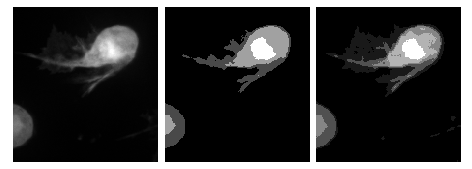
\includegraphics{img/fig_kmeans}
	\caption{Application of the K-Means algorithm to a test image. \textbf{Top left}: Input image. \textbf{Top right}: Ground truth labels of the input image. \textbf{Bottom left}: K-means results with $k=4$,  using arbitrary colors for the labels. \textbf{Bottom right}: Results with $k=6$. It is noteworthy that while the results for $k=4$ are reasonable, the nearly transparent lamellopodium pixels are labelled as background values, while the cell proper is segmented into two parts.}
	\label{fig:kmeans}
\end {figure}

\noindent Obviously, this algorithm can also be used to segment images into $k$ different classes, but since K-Means assigns classes to data by using the distance from the mean, the algorithm output favors segmentations in which the classes have roughly the same size, which isn't necessarily the correct way to classify pixels in arbitrary image data.

	\section{Canny Edge Detection}
The \textit{Canny Edge Detector} \cite{canny} is one of the most famous edge-detection algorithms and actually is a composite algorithm that returns a binary segmentation of an image into edges and non-edges.\\

\noindent First, a Gaussian convolution filter is applied to try and subdue noise in the image. A \textit{convolution} is a matrix operation often used in image processing: A matrix $A$, describing the pixel values of an image, is convolved pixel-wise with a convolution matrix $B$ with dimensions $n \times n$ - that is, for each pixel $p$ of $A$, the pixel's $n \times n$-neighborhood pixel values are summed up while being weighted according to corresponding value in $B$. The resulting sum is then assigned to the output matrix in place of the previous value of the center pixel, which intuitively assumes the distance-weighted average value of its neighborhood. In the case of pixels that lie on the edge of the matrix to be convoluted, out-of-bounds considerations have to be made: A constant value such as zero can be assumed for the pixels in the neighborhood that would lie ``outside'' of the image, the existing image values can be mirrored or clamped to provide a torus-like out-of-bounds handling, or the convolution can be done only on those pixels whose neighborhood fully lies inside of the image, resulting in smaller output images.

The aforementioned ``Gaussian filter'' or ``kernel'' is a matrix whose values are defined so that performing a convolution using that matrix approximates the behavior of the two-dimensional Gaussian function with uniform variances for its $x$- and $y$-dimensions:

\[ f(x, y) = \exp \left(- \left( \frac{\left(x - p_x \right)^2}{2\sigma^2} + \frac{ \left(y - p_y \right)^2}{2\sigma^2} \right) \right), \]

\noindent where $p$ is the center pixel of the current neighborhood. Subsequently, $p_x$ and $p_y$ are the coordinates of this pixel within the matrix and $\sigma$, the standard variance, acts as the smoothing constant. The higher this constant is, the stronger the blur effect becomes.

In Gaussian filters, the $\sigma$ constant is expressed through the dimensions of the matrix - the larger the filter matrix, the stronger the blur effect. An example for a $3 \times 3$ Gaussian filter is the following matrix:

\[ \frac{1}{16} \left [ \begin{tabular}{ccc}
				1& 2& 1\\
				2& 4& 2\\
				1& 2& 1 
			   \end{tabular} \right ]\]

\noindent The coefficient $\frac{1}{16}$ is equal to the sum of the matrix values and ensures that the convolution does not change the average image value. \cite[p. 41]{machine_vision}\\

\noindent As the second step, an gradient-based edge detector filter is applied to the smoothed image. The most famous of these is the \textit{Sobel filter} \cite{sobel}, which approximates the local partial derivatives $\frac{\partial I}{\partial x}$ and $\frac{\partial I}{\partial y}$ of each pixel of the image function $I(x, y)$, using the $3 \times 3$ neighborhood of that pixel. It is given by the following matrices\cite[pp. 113 -- 114]{machine_vision}:

\[ \text{Sobel}_x = \left [ \begin{tabular}{ccc}
				-1& 0& 1\\
				-2& 0& 2\\
				-1& 0& 1 
			   \end{tabular} \right ] \text{ and } 
\text{Sobel}_y = \left [ \begin{tabular}{ccc}
				1& 2& 1\\
				0& 0& 0\\
				-1& -2& 1 
			   \end{tabular} \right ] 
\]

\noindent The result of these convolutions are two images, $G_x$ and $G_y$, which represent the partial local derivatives of each pixel. The gradient image of the original input image $I$ is then defined as

\[G = |\nabla I| = \sqrt{{G_x}^2 + {G_y}^2}.\]

\noindent Additionally, the gradient direction of each pixel can be calculated from the derivative images by measuring the angle between the x-axis and the gradient pixel coordinates by employing the atan2 function:

\[G_\phi = \text{atan2}(G_y, G_x) \]

\noindent Using $G_\phi$, edge thinning via non-maximum suppression is applied to the gradient image as the third step in the algorithm: For each pixel, the gradient direction acts as a criterion to decide which two neighboring pixels, that are each on opposite sides (positive and negative direction of the gradient), should be compared to the current pixel. If the value of the current pixel is not larger than the two neighbors' values, the pixel's value is not a local maximum and is set to zero. The gradient direction angles can either be rounded so that each angle represents one of the north-south, west-east directions and so forth, or linear interpolation can be used.

In the final step, a hysteresis threshold is applied. This process consists of defining two thresholds, $\theta_{high}$ and $\theta_{low}$. The definition for the thresholding function as given in \ref{sec:thresholding} is slightly altered:

\[ T(I(x, y), \theta_{high}, \theta_{low}) =  \begin{cases}
							2 \text{ if } I(x, y) \, \geq \, \theta_{high} \\
							1 \text{ if } I(x, y) \, \geq \, \theta_{low} \text{ and } < \theta_{high} \\
			          				0 \text{ otherwise}
			   			        \end{cases}
\]

\noindent Pixels that have a value of $2$ are called strong pixels because they had values larger than the high threshold, whereas pixels with a value of $1$ are called weak pixels. Finally, the algorithm checks for each pixel if an 8-connected path between that pixel and a strong pixel exists - if not, then the pixel is dropped. This can be done with the help of connected component-finding algorithms by dropping each ``$1$''-component which is not connected to at least one ``2''-value.\\

\noindent The thresholds $\theta_{high}$ and $\theta_{low}$ have to be set by the user, although there exists the possibility to set these by using the Otsu threshold described in \ref{sec:thresholding} . Using this combination approach, $\theta_{high}$ is set to the Otsu threshold value for $I(x, y)$, and $\theta_{low}$ is set to $0.5 * \theta_{high}$.\cite{otsu_combine}


	\section{Gaussian Mixture Models}
Gaussian Mixtures Models (GMMs) are a subclass of mixture models, that is, probabilistic models which are combined with other models of the same distribution type to form a more complex model that is able to model the distribution of a data set more accurately than a simple model could. In the case of GMMs, the base distributions are often $n$-multivariate Gaussian distributions:

\[ pdf(x) = \mathcal{N}_n (x\,|\,\mu,\, \Sigma) \]

\noindent Here, $pdf(x)$ denotes the probability, or density, of an $n$-dimensional piece of data $x$, while $\mu$ and $\Sigma$ are the $n$-dimensional mean vector and the $n \times n$ covariance matrix of the distribution. Since the shape such a distribution can take is limited, a single Gaussian cannot accurately model a multimodal distribution (see Figure \ref{fig:normal_vs_gmm}). Instead, a weighted combination of multiple Gaussians can be used instead: \cite[pp. 430]{bishop_pattern}

\[ pdf_m (x) = \sum \limits_{k=1}^{K} \pi_k \, \mathcal{N}_n (x\,|\, \mu_k, \Sigma_k) \]

\noindent A mixture model consists of $K$ models that each have different parameters $\mu$ and $\Sigma$ and are weighted by weights $\pi_k \in \mathbb{R}$, $1 > \pi_k > 0$, with $\sum_{i=1}^{k} \pi_i = 1$.

\begin {figure}[!ht]
	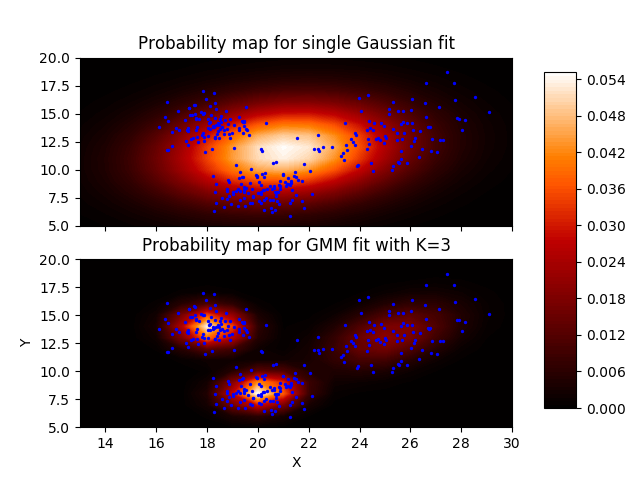
\includegraphics{img/fig_normal_vs_gmm}
	\caption{Comparison of a single Gaussian fit (upper) with a GMM fit, using $K=3$, on a two-dimensional dataset randomly sampled from three Gaussian distributions. The single Gaussian fails to capture the structure of the data, while the GMM succeeds.}
	\label{fig:normal_vs_gmm}
\end {figure}

\noindent The parameters of such a mixture model can be calculated by applying the Expectation-Maximization (EM) algorithm, which can additionally be combined with a K-Means initialization to avoid shallow local minima.\cite{em_algorithm} GMMs can also be used for segmenting images: Grayscale images are simply three-dimensional data in which each pixel coordinate corresponds to an intensity value. If the number of components to be found in the image is known beforehand, as it is in the case of cell segmentation, the intensity values can be segmented according to the fitted GMM (see Figure \ref{fig:gmm_vs_gt}). To do this, for each pixel in the image the posterior probabilities for that pixel in respect to each of the Gaussians is calculated and the Gaussian with the highest probability is chosen as the ``source'' of the pixel:

\[ label_x = \argmax \limits_{k} \, p(\mu_k, \Sigma_k\, | \, x) \]

\begin {figure}[!ht]
	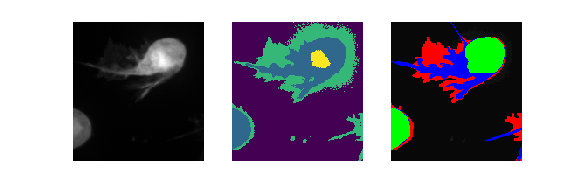
\includegraphics{img/fig_gmm_vs_gt}
	\caption{From left to right: Input image, pseudo-color labels assigned by a $K=4$ GMM fit to the input image and the ground truth labels for the input image.}
	\label{fig:gmm_vs_gt}
\end {figure}


	\section{Graph Cuts}



	\section{Multi-layer Perceptrons}
\textit{Multi-layer Perceptrons} (MLPs) or \textit{Feedforward Artificial Neuronal Networks} (ANNs) are mathematical functions that try to emulate the way neurons in the brain process information, typically to classify data or perform regression on it. ANNs have recently achieved impressing results on various tasks, such as image classification, sound analysis and regression, typically achieved by very deep networks that used lots of artificial neurons and were fed large datasets exceeding one million samples. In this section, the concepts behind optimization of functions via Gradient Descent, neuronal networks and training of those networks using the Backpropagation algorithm are explained. 



\subsection {Gradient Descent}
\textit{Gradient Descent} or the ``method of steepest descent'' is a standard, analytic first-order technique first introduced by that can be used to minimize or maximize at least once-differentiable functions, that is, to calculate a vector of parameters $\Theta$ for a function $f$ so that

\[ \Theta = \argmax \limits_{i} f(i) \]

\noindent To find values for $\Theta$, the approach takes advantage of the fact that the negative gradient vector $\nabla_f = [ \frac{\partial f}{\partial \Theta_0}, \dots, \frac{\partial f}{\partial \Theta_n} ]$, the vector of all first partial derivatives of $f$, points into the direction of the fastest change, or put graphically, the ``steepest slope''. By taking steps into the direction of this gradient, the function value is minimized step by step, while maximization works the same, only that the function is negated and then minimized, which results in parameters that maximize the original function. The parameter $\eta$ depicts the step size and is typically a value in the range $(0.0, 1.0]$. \cite[pp. 40--42]{optimization_book}

The algorithm starts with a guess for the parameters in $\Theta$ and then iteratively evaluates the gradient and updates the parameters accordingly until convergence within arbitrary precision is reached (see algorithm \ref{alg:grad_desc}).

\begin {algorithm}
	\begin {algorithmic}[1]
		\State $\Theta_0$ = random
		\While {$|f(\Theta_i) - f(\Theta_{i - 1})| > \epsilon$}
			\State $\Theta_i = \Theta_{i-1} - \eta \nabla_f$ 
		\EndWhile
	\end{algorithmic}
	\caption{Gradient Descent scheme for optimizing differentiable functions.}
	\label{alg:grad_desc}
\end{algorithm}

\noindent For convex functions, Gradient Descent always finds the global minimum. For non-convex functions however, the algorithm may get stuck in a local minimum or at saddle points, called ``false minima' (see figure \ref{fig:grad_desc}). Therefore, running the algorithm multiple times with random values or even informed guesses given knowledge about the form of the function to be optimized is advised. The step size $\eta$ has to be chosen depending on the shape of the function to minimize; if $\eta$ is too large, the algorithm will overshoot the minimum and never converges, even if the minimum exists, and if $\eta$ is too small, convergence will take a long time. Also, for some functions, the algorithm starts moving in a zig-zag pattern near the optimum, further increasing the number of steps the algorithm takes until covergence. To address these problems, a number of optimizations were proposed, some of which are discussed in section \ref{chapter_optimization}.


\begin {figure}[!ht]
	\begin{center}
		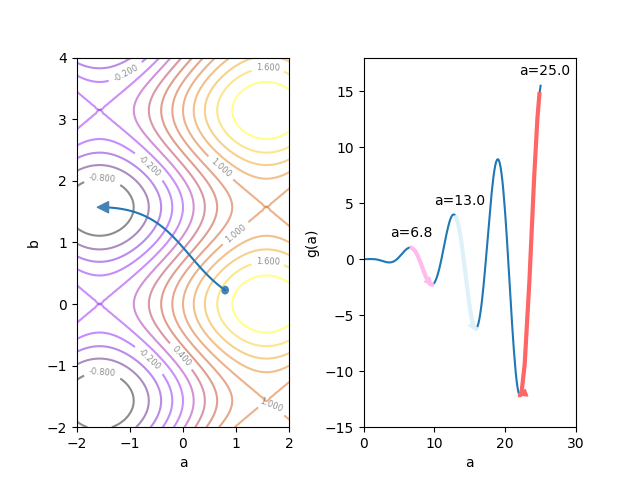
\includegraphics[scale=0.9]{img/fig_grad_desc}
	\end{center}
	\caption{\textbf{Left:} A contour plot of Gradient Descent minimization of $f(a, b) = \sin(a) + \cos^2(b)$. The blue line shows the search path of the algorithm along the negative gradient while estimating the optimal $\Theta$. \textbf{Right}: Effect of the initial guess for $\Theta$ on the optimization. The function $f(a) = \frac{1}{40}a^2 * \frac{1}{2} \cos(a)$ has multiple local minima in the interval [0, 25]. Only the third guess $a=25$ leads to finding the global minimum, while the other two optimization runs get trapped in local minima.}
	\label{fig:grad_desc}
\end {figure}


	\subsection{The Perceptron Algorithm}
A single-layer ANN is a network consisting of just one neuron, and is also called ``perceptron''. The idea for the perceptron was first proposed by Rosenblatt \cite{rosenblatt_report, rosenblatt_book}, who used it to perform binary classifications, using what is now called the ``perceptron algorithm''. Given a linearly separable set of $m$ data points of dimension $n$, one can construct a $(n+1) \times m$ input matrix $x$. The last entry in every column is set to $1$.

The \textit{perceptron classifier}, the function that decides which class a given sample belongs to, then takes the form of a linear function

\[ d(x) = f(w^{T}x), \]

\noindent where $w$ is a vector of dimension $n+1$ and contains the $n$ \textit{weights} and the \textit{bias} value. The function $f$ is the \textit{activation function}, which is defined as 

\[ f(a) =  \begin{cases}
		+1 \text{ if } a \geq 0 \\
	   	 -1 \text{ otherwise}
	    \end{cases}\]

\noindent and maps its input to one of two possible classes.

The task of the \textit{training phase} is to find values for $w_0, \dots, w_{n+1}$ so that each data point is classified correctly by the resulting line, plane or (hyper-)plane. To this account, there needs to be a $m$-dimensional vector $t$ containing the \textit{labels} of each data point to verify the correctness of $w$. These labels are integers that indicate which class each data point belongs to. In the case of the perceptron algorithm, the labels are either $1$ for the first class $C_1$ or $-1$ for the second class, $C_2$. If all data points are classified correctly by some $w$, then it holds that

\[ w^T x_n \, t_n > 0 \,\,\forall\, x_n \in x \label{eq:perceptron_label} \]

\noindent Using this definition of correctness, a correctness measure or \textit{error function} can be formulated, which is known as the ``perceptron criterion''. It is given by

\[ E_p(w) = - \sum \limits_{n \in \mathcal{M}} w^T x_n\, t_n, \label{eq:perc_error}\]

\noindent where $\mathcal{M}$ is the set of all data points that were misclassfied, meaning that evaluating equation \ref{eq:perceptron_label} for that data yields a value $< 0$. \cite[pp. 192--194]{bishop_pattern}\\

\noindent The correct perceptron weights can then be determined by some arbitrary learning algorithm, although here, the Gradient Descent scheme (see algorithm \ref{alg:grad_desc}) is applied to the error function \ref{eq:perc_error}. When optimizing functions that not only depend on the parameters $\Theta$ but also on some dataset, one can consider one of the subtypes of Gradient Descent; either, evaluating the average gradient using all available data samples (\textit{Batch Gradient Descent}) or using single data points only - as an approximation of the entire dataset - to perform the updates. This is called \textit{Stochastic Gradient Descent} (SGD) and is preferable if working with datasets that are too large to fit into memory. Alternatively, one can use the average gradient of a subset of data points - this method is often referred to as \textit{Mini-Batch} Gradient Descent.

Either way, the gradient of $E_p$ has to be calculated. The perceptron criterion only depends on the weights $w$, so the gradient vector has the shape

\[ \nabla_E = \left[ \frac{\partial E_p}{\partial w_0}, \frac{\partial E_p}{\partial w_1}, \dots, \frac{\partial E_p}{\partial w_{n+1}} \right ] \].

Taking the partial derivatives in respect to $w$ leads to

\begin{align}
 	\hspace{2em}&\hspace{-2em} \nabla_E = \frac{\partial E_p}{\partial w} = \frac{\partial}{\partial w} \left (- \sum \limits_{n \in \mathcal{M}} w^T x_n t_n \right ) \\
 	&= -\sum \limits_{n \in \mathcal{M}} x_n t_n
\end{align}

\noindent If SGD is used, this is reduced to simply

\[ \nabla_E = -x_n t_n\]

\noindent for some previously misclassified point $x_n \in \mathcal{M}$ in the dataset. Hence, the update rule for the perceptron becomes

\[w_i = w_{i - 1} + x_n t_n * \eta\]

\noindent Using this update rule leads to the training algorithm shown in \ref{alg:perceptron_algorithm}, which is applied to an example dataset in figure \ref{fig:perceptron}.

\begin {figure}[!ht]
	\begin{center}
		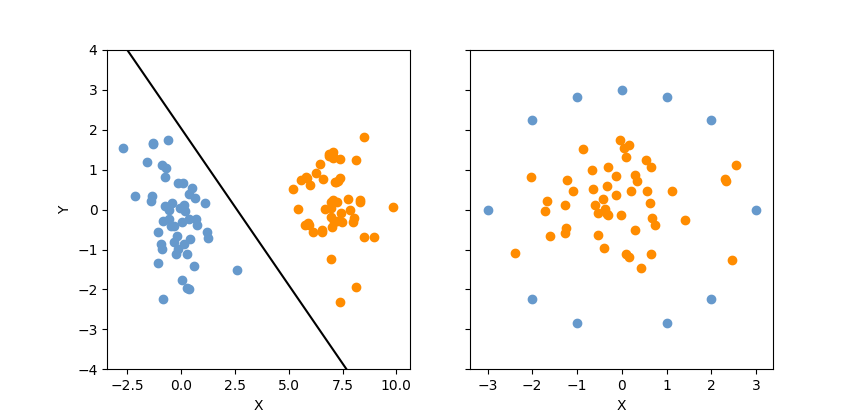
\includegraphics[scale=0.6]{img/fig_perceptron}
	\end{center}
	\caption{\textbf{Left}: Separating two datasets with the perceptron algorithm in $\mathbb{R}^2$. The correct classification boundary takes the form of a line, i.e. $0 = w^{T}x = w_0 x + w_1 y + w_2$. The line pictured is given by $w = (-2.285, -2.908, 5.938)$, the weights after 19 iterations. \textbf{Right}: A not-linearly separable data set, on which the algorithm would never converge, because it is based on finding linear classifiers and thus cannot separate the data correctly.}
	\label{fig:perceptron}
\end {figure}

\begin {algorithm}
	\begin {algorithmic}[1]
		\State $w$ = random
		\While {true}
			\For{$x_i$ in $x$}
				\If{$w^T x_i t_i \leq 0$}
					\State $w$ += $x_i t_i * \eta$
				\EndIf

				\If{$w^T x_i t_i > 0$ for all $x_i$ in $x$}
					\State stop
				\EndIf
			\EndFor
		\EndWhile
	\end{algorithmic}
	\caption{Stochastic Gradient Descent applied to the task of finding the perceptron weights $w$. $x$ is assumed to be linearly separable.}
	\label{alg:perceptron_algorithm}
\end{algorithm}



		\subsection{Multiple Neurons and Backpropagation}
While the perceptron algorithm works fine for linear problems, those are only a small subset of real-world problems: Even the simple problem of learning to classify the XOR dataset obviously cannot be solved by the perceptron. The solution to this problem is to add more neurons to the model, which form a network that consists of layers that pass the outputs of neurons in the previous layers through non-linear activation functions and then use the results as inputs. These layers are referred to as the ``input layer'', the first layer, the ``output layer'', the last layer, and ``hidden layers'', which are all the layers inbetween.

The resulting networks are called \textit{Multi-Layer Perceptrons} (MLPs), \textit{Feedforward Artificial Neural Networks}(ANNs), or, in the case of a multitude of layers, \textit{Deep Neural Networks}, and are much more powerful than simple perceptrons, as they can approximate haphazard continuous functions that operate on closed and bounded subsets of $\mathbb{R}^n$ given that the network possesses at least one hidden layer of neurons. This capability makes using MLPs for learning real-life problems feasible.\cite{universal_approx}\cite{universal_approx2}\\

\noindent Mathematically, the outputs $out_k$ of an MLP can be defined as follows:

\[  out_k(x, w) = \sigma \left( \sum \limits_{a=1}^{D^{(n)}} w_{ka}^{(n)} \cdot h \left ( \,\dots\, h\left ( \sum \limits_{z=1}^{D^{(1)}} w_{yz}^{(1)} x_{z^{(1)}} + w^{(1)}_{0} \right ) \dots \right ) + w_{0}^{(n)} \right ) \]

\noindent where \textbf{$x$} is the vector of inputs and \textbf{$w$} is a matrix of weights. \textbf{$D$} is equal to the number of inputs to a layer, while \textbf{$h$} denotes an activation function and \textbf{$\sigma$} is an output function. The superscripts denote which layer in the network a variable refers to. The weights $w$ are doubly indexed with the index of the neuron in the next layer to which the function that uses the weights is the input as well as the index of the layer they belong to. For example, a weight $w_{12}$ refers to the vector of weights of the second layer that parametrizes the input function to the first neuron in the successive, third layer. The running variables within each layer are written as \textbf{$a \dots z$}, with \textbf{$a$} denoting the variable for the inputs of the first layer and \textbf{$z$} is used for the inputs of the last layer; all layers in between are defined accordingly.\\

\noindent The choice of the activation function $h(w, x)$ is different from the normal perceptron: It is not chosen to be the Heaviside function, but instead, to be a non-linear, continuous and differentiable function. Computing an output is done by passing the input vector to the first layer, which computes its activations for all its neurons, which then pass on their activations to the neurons of the next layer as inputs until the output layer is reached.

The output function $\sigma$ is applied in the last layer of the network, and is dependent on the task the network is supposed to fulfill: For regression problems, fitting a function to a set of data and then predicting new values using that function, the identity function can be used, but for binary classification problems, instead of using a step function like in the original perceptron, one instead uses the continuous sigmoid function and interprets the output as

\[ sigmoid(x_i, w) =  \begin{cases}
				x_i \in C_1 \text{ if } sigmoid(x_i, w) \geq 0.5 \\
				x_i \in C_2 \text{ else }\\
			 \end{cases}
\]

\noindent If the classification is non-binary, using the softmax function (see section \ref{subsec:softmax}) to obtain probabilities for the likeliness of $x_i$ being in any of the classes is a solution. 

